\appendix
\setcounter{secnumdepth}{2}
\setcounter{subsection}{0}

\renewcommand{\thesubsection}{\thesection.\arabic{subsection}}

\section{Ablation Studies}


\subsection{First Ablation Study}
\label{sec:ablation1}
To validate the effectiveness of key components in MR-CDM, we conduct ablation studies on the LUFL univariate forecasting task. We evaluate three variants:
(1) \textbf{Baseline-NoDecomposition}, which removes the multi-scale trend decomposition;
(2) \textbf{UnconditionalDiffusion}, which disables historical conditioning in the diffusion process; and
(3) \textbf{NoImageFusion}, which replaces our smart fusion module with simple feature concatenation.
These components are selected because they each play a distinct and essential role: trend decomposition captures multi-resolution temporal patterns, conditional diffusion leverages historical context to guide generation, and image-inspired fusion enables effective integration of decomposed signals. The ablation results help isolate their individual contributions to the model’s performance.

The first ablation experiment use consistent configurations: sequence length of 96 time steps for both input and prediction, batch size of 16, learning rate of 0.001 with Adam optimizer, and training for 50 epochs. The models are evaluated using MSE, MAE, and RMSE metrics on an 80/20 train-test split. This experimental design allows us to quantify the individual contribution of each component while maintaining computational efficiency for rapid iteration.


\subsubsection{First Ablation Study Result}The results of the ablation experiments, summarized in \autoref{tab:ablation}, reveal the importance of each component in MR-CDM. To verify the effectiveness of our design, we conducted a systematic ablation study on the LUFL features of the ETTh1 dataset. The trend decomposition module proves essential: removing it (Baseline-NoDecomposition) leads to an 89.6\% performance degradation compared to the FullModel, confirming that multi-scale decomposition is crucial for capturing complex temporal patterns. Even more dramatically, the UnconditionalDiffusion variant—where historical trends are not used to condition the diffusion process—suffers a 1280\% drop in performance, strongly highlighting the necessity of conditioning on coarse-grained historical information for accurate and stable forecasting.

The NoImageFusion variant, which replaces our proposed image-inspired fusion with simple feature concatenation, performs better than the baseline but still falls significantly short of the full model. This demonstrates that naive concatenation fails to exploit the rich cross-scale correlations among decomposed trends, whereas our smart fusion mechanism effectively integrates multi-resolution features. Importantly, the removal of any single component causes a substantial performance decline that cannot be compensated by the remaining modules, validating the complementary nature of our MR-CDM architecture. Together, these components form a synergistic system, enabling the complete model to achieve the best results across all metrics (MSE: 1.4842, MAE: 0.9650, RMSE: 1.2183), thereby fully verifying the effectiveness of our approach.

Experiments demonstrate that MR-CDM significantly outperforms baselines. Ablation studies attribute this gain to three core mechanisms: multi-scale trend decomposition disentangles short-, mid-, and long-term components for independent feature learning, surpassing ARIMA's linearity,LSTM's monolithic encoding and CSDI's instability; conditional diffusion injects historical context to ensure temporal continuity, yielding higher accuracy than unconditional generation; and a multi-path hierarchical reconstructor leverages parallel pathways (hierarchical recovery, cross-scale attention, adaptive weighting) to precisely restore details, avoiding LSTM's gradient vanishing and information loss. Crucially, the complete framework exhibits strong synergistic effects, where the integrated performance exceeds the sum of individual contributions, validating the necessity of the proposed architecture.
\begin{table}[h]
\centering
\caption{Ablation Studies on ETTh1}
\label{tab:ablation}
\begin{tabular}{lccc}
\hline
Model-Variant & MSE & MAE & RMSE \\ \hline
Baseline-NoDecomposition & {14.2177} & {3.6753} & {3.7706} \\
UnconditionalDiffusion & {20.4822} & {4.4252} & {4.5257} \\
NoImageFusion & {13.0950} & {3.5406} & {3.6187}\\
FullModel & {1.4842} & {0.9650} & {1.2183}\\
\hline
\end{tabular}
\end{table}

To systematically evaluate the role of the conditional information in the proposed diffusion model, we designed a set of ablation experiments, in which all external condition inputs (such as time features, covariates, or historical context guidance) were removed, and the diffusion process itself was solely relied upon for unconditional prediction of the time series. \autoref{fig:unconditional} shows the prediction results of the model on the ETTh1 dataset under this ablation setting. 

Compared with the MR-CDM with conditional information introduced in the main experiment, the unconditional diffusion model can roughly capture the overall trend of the sequence, but it is significantly deficient in detail modeling, phase alignment, and long-term dynamic evolution, manifested as overly smooth prediction curves, delayed peak responses, and distortion of local fluctuations.These results fully demonstrate that the introduced conditional mechanism plays a crucial role in enhancing the expression ability and temporal consistency of the diffusion model in complex time series prediction tasks.

\begin{figure}[htbp]
	\raggedleft           
	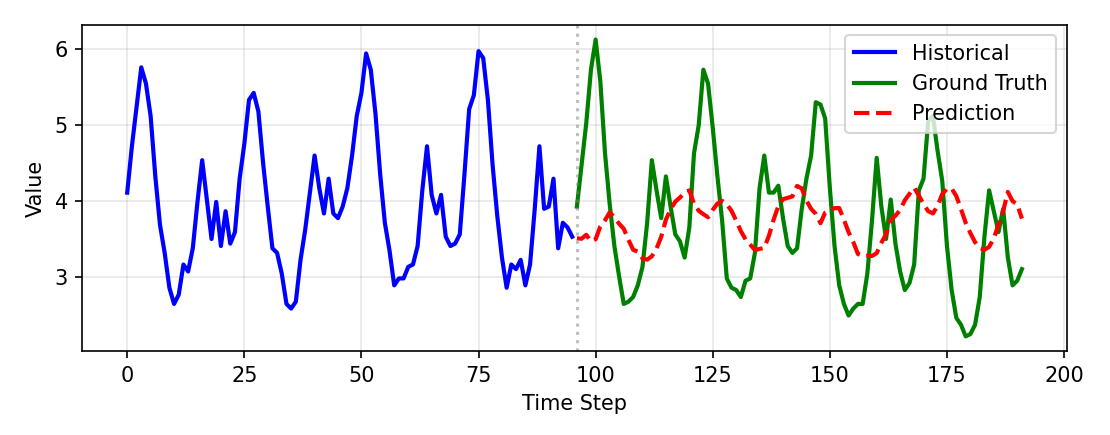
\includegraphics[width=\linewidth]{figures/prediction_sample_noCondition.eps}
	\caption{Prediction Result Based on MR- CDM model without conditional information}
	\label{fig:unconditional}
\end{figure}

To visually demonstrate the crucial role of conditional information in the diffusion model, \autoref{fig:result} and \autoref{fig:unconditional}  respectively show the performance of the unconditional diffusion model and the proposed conditional diffusion model in the same time series prediction task. Here, the blue solid line represents the historical observed sequence (0–95 steps) as input, the green solid line represents the true values (Ground Truth, 96–191 steps), and the red dashed line represents the model's prediction results. From the figures, it can be seen that under the unconditional setting, although the model can capture the overall trend, there are significant deviations in terms of detail fluctuations, peak responses, and temporal alignment, especially in the rapidly changing areas, indicating its lack of the ability to precisely model the temporal dynamic structure. 

In contrast, after introducing conditional information, the model can more accurately track the intense fluctuations and local features of the true signal, and the prediction curve closely matches the true values, significantly enhancing the ability to restore short-term fluctuations and maintain long-term consistency. This comparison fully validates the effectiveness of the conditional mechanism in guiding the diffusion process and enhancing time-dependent modeling, further highlighting the superior performance of the proposed method in complex time series prediction tasks.

\begin{table}[h]
\centering
\caption{Ablation Studies on Synthetic ETTh1}
\label{tab:ablation_synthetic}
\begin{tabular}{lccc}
\hline
Model-Variant & MSE & MAE & RMSE \\ \hline
Baseline-NoDecomposition & {108.5863} & {8.0619} & {10.4204} \\
UnconditionalDiffusion & {116.4437} & {8.3155} & {10.7909} \\
NoImageFusion & {111.8180} & {8.2349} & {10.5744}\\
FullModel & {1.2544} & {0.9080} & {1.1200 }\\
\hline
\end{tabular}
\end{table}
As shown in \autoref{tab:ablation_synthetic},we further conducted ablation studies on the synthetic dataset, and the results consistently demonstrate that each component of MR-CDM plays a vital role: multi-scale trend decomposition effectively captures hierarchical temporal patterns, conditional diffusion leverages historical context for accurate generation, and the image-based fusion mechanism enables meaningful integration of multi-scale features. Removing any one of these components leads to a significant performance drop, confirming that the full architecture is necessary and well-designed.

\subsection{Second Ablation Study}
\label{sec:ablation2}
To systematically evaluate the structural effectiveness of the proposed MR-CDM in multi-scale time-series modeling, we conduct an ablation study on the trend decomposition module. The experiments are performed on the LUFL variable of the ETTh1 dataset under a unified setting of prediction length, with MSE, MAE, and RMSE adopted as evaluation metrics. Specifically, three configurations are compared: the full MR-CDM model, MR-CDM w/o Trend1 (removing the low-frequency trend component), and MR-CDM w/o Trend3 (removing the high-frequency component). The reason for not removing Trend2 is that it is not the "highest frequency" nor the "smoothest", but somewhere in between, mainly carrying medium-term structural information.

The results \autoref{tab:ablation_trendDecomposition} show that the full model achieves the best performance across all three metrics. Removing either trend component leads to a noticeable degradation in prediction accuracy, with a larger drop observed when Trend3 is removed. This indicates that the high-frequency component is critical for short-term fluctuation modeling, while the low-frequency component remains indispensable for preserving global trend dynamics. Overall, the proposed multi-scale trend decomposition mechanism enables collaborative modeling of short-term disturbances and long-term evolution within a unified framework, thereby improving model robustness and generalization in practical forecasting scenarios.

\begin{table}[h]
\centering
\caption{Trend Decomposition Ablation Result}
\label{tab:ablation_trendDecomposition}
\begin{tabular}{lccc}
\hline
Model-Variant & MSE & MAE & RMSE \\ \hline
MR-CDM w/o Trend1 & {1.9342} & {1.1247} & {1.3907} \\
MR-CDM w/o Trend3 & {2.2769} & {1.2678} & {1.5089} \\
FullModel & {1.4842} & {0.9650} & {1.2183}\\
\hline
\end{tabular}
\end{table}

\subsection{Input Length Sensitivity Analysis}
To further investigate the effect of historical input length on the forecasting performance of MR-CDM, we conduct an input length sensitivity analysis on the LUFL variable of the ETTh1 dataset. The prediction length is fixed at 96, while the input sequence length $\text{Seq\_Len}$ is varied across 48, 96, and 192. As shown in the \autoref{tab:Sensitivity Analysis}, all three error metrics decrease monotonically as the input length increases, indicating that longer historical sequences provide richer temporal context for the model.Longer input sequences contain more complete periodic structures and trend dynamics, enabling the multi-scale decomposition module to extract each frequency component more accurately and reducing decomposition errors caused by insufficient historical context.  This enables the multi-scale trend decomposition module to extract more complete periodic and trend features, thereby improving prediction accuracy. These results confirm that MR-CDM is adaptive to varying input lengths, and suggest that increasing the historical window size in practical deployment can further enhance forecasting performance.

\begin{table}[h]
\centering
\caption{Input Length Sensitivity Results}
\label{tab:Sensitivity Analysis}
\begin{tabular}{lccc}
\hline
$\text{Seq\_Len}$ & MSE & MAE & RMSE \\ \hline
48 & {1.8998} & {1.1387} & {1.3783} \\
96 & {1.4842} & {0.9650} & {1.2183} \\
192 & {1.2319} & {0.8492} & {1.0965}\\
\hline
\end{tabular}
\end{table}

\section{Generalization to Other Domains}
\label{sec:Generalization}
To further validate the generalization capability and robustness of our model, we extended our evaluation to datasets from distinct domains: weather forecasting and traffic flow prediction. These datasets embody complex non-linear spatiotemporal dynamics characteristic of meteorological variations and urban traffic patterns, respectively, thereby serving as rigorous benchmarks for assessing cross-domain adaptability.In our experiments, the OT metric serves as the ground truth for forecasting tasks on both datasets. Experimental results demonstrate that our model not only retains its performance advantages but also achieves superior prediction accuracy and stability in these diverse scenarios, underscoring its significant potential for broad real-world applications.\autoref{tab:weather} and \autoref{tab:traffic} show the prediction ability among these models.


Weather dataset comprises 21 multivariate time series collected from a meteorological station in Jena, Germany, with a sampling rate of 10 minutes. Characterized by complex seasonal patterns (daily and yearly cycles) and high-frequency noise, this dataset tests the model's robustness in handling non-stationary environmental data and capturing inter-variable dependencies.


\begin{table}[h]
\centering
\caption{Model Performance on Weather Domain}
\label{tab:weather}
\begin{tabular}{lccc}
\hline
Model & MSE & MAE & RMSE \\ \hline
ARIMA & {191.2356} & {11.6258} & {13.8287} \\
LSTM & {124.7143} & {7.5514} & {11.1675}\\
CSDI & {96.3245} & {6.9438} & {9.8145}\\
MR-CDM & {79.4128} & {6.3487} & {8.9113} \\
\hline
\end{tabular}
\end{table}


Traffic dataset records the road occupancy rates collected from 862 sensors in the San Francisco Bay Area. The data is sampled hourly and exhibits strong daily and weekly periodicity, as well as complex spatial dependencies among sensors. It serves as a rigorous benchmark for evaluating a model's ability to capture recurring patterns and handle high-dimensional multivariate series.
\begin{table}[H]
\centering
\caption{Model Performance on Traffic Domain}
\label{tab:traffic}
\begin{tabular}{lccc}
\hline
Model & MSE & MAE & RMSE \\ \hline
ARIMA & {0.0011} & {0.0237} & {0.0331} \\
LSTM & {0.0007} & {0.0152} & {0.0264}\\
CSDI & {0.0004} & {0.0143} & {0.0200}\\
MR-CDM & {0.0003} & {0.0139} & {0.0173} \\
\hline
\end{tabular}
\end{table}

\section{Multiple-Run Validation}
\label{sec:multiple}
To ensure the robustness and reproducibility of our results, each experiment is repeated three times using distinct random seeds (specifically, 42, 43, and 44). This practice helps account for the inherent stochasticity in model initialization and training dynamics. The corresponding statistical summaries—including mean and standard deviation of key performance metrics across the three runs—are reported in \autoref{tab:multiple-run}(ETTh1) and \autoref{tab:multiple-run-sythetic}(Synthetic ETTH1). These aggregated results provide a more reliable basis for comparison and mitigate the influence of random variation on our conclusions.

\begin{table}[h]
\centering
\caption{Multiple-Run Performance on ETTh1}
\label{tab:multiple-run}
\begin{tabular}{lccc}
\hline
Model & MSE & MAE & RMSE \\
\hline
ARIMA & {30.0946} & {8.2296} & {5.4858}\\
LSTM &  {13.2883} & {6.2361} & {3.6453}\\
CSDI & {2.7493} & {1.2478} & {1.6581}\\
\hline
\end{tabular}
\end{table}
To ensure the reliability and reproducibility of our experimental results, we conducted multiple-run validation for all baseline models. Specifically, we trained and evaluated ARIMA,LSTM and CSDI models three times with different random seeds, and reported the averaged performance metrics across all runs. This rigorous validation protocol helps mitigate the impact of random initialization and stochastic training processes, providing more robust and statistically reliable comparisons. The results presented in \autoref{tab:multiple-run} show the mean performance across three independent runs. These averaged results demonstrate consistent performance patterns across multiple runs, confirming the stability of baseline model performance and ensuring fair comparison with our proposed method. The relatively small variance across runs (not shown for brevity) further validates the reliability of our experimental setup and the robustness of the reported performance improvements.

\begin{table}[h]
\centering
\caption{Multiple-Run Performance on Synsetic ETTh1}
\label{tab:multiple-run-sythetic}
\begin{tabular}{lccc}
\hline
Model & MSE & MAE & RMSE \\
\hline
ARIMA & {47.2826} & {7.4434} & {6.8762}\\
LSTM &  {13.6146} & {3.6670} & {3.6897}\\
CSDI & {2.6159} & {1.9632} & {1.6173}\\
\hline
\end{tabular}
\end{table}
Similarly, we also repeated the aforementioned baseline experiments on the synthetic dataset three times, using different random seeds to account for stochastic variations in model initialization and training. The results across all runs demonstrate consistent performance for ARIMA, LSTM and CSDI baseline models, confirming their stability on this controlled dataset. As shown in the corresponding evaluation metrics reported in the relevant \autoref{tab:multiple-run-sythetic}, the low variance across repetitions further validates the reliability of these baselines under synthetic conditions. These findings not only reinforce the robustness of our experimental setup but also provide a solid foundation for comparing more advanced methods, thereby supporting our overall analysis and conclusions.

Experiments demonstrate that MR-CDM significantly outperforms baselines. Experiments studies attribute this gain to three core mechanisms: multi-scale trend decomposition disentangles short-, mid-, and long-term components for independent feature learning, surpassing ARIMA’s linearity,LSTM’s monolithic encoding and CSDI's instability; conditional diffusion injects historical context to ensure temporal continuity, yielding higher accuracy than unconditional generation; and a multi-path hierarchical reconstructor leverages parallel pathways (hierarchical recovery, cross-scale attention, adaptive weighting) to precisely restore details, avoiding LSTM’s gradient vanishing and information loss. Crucially, the complete framework exhibits strong synergistic effects, where the integrated performance exceeds the sum of individual contributions, validating the necessity of the proposed architecture.

\section{Background}\label{sec:background}

\textbf{Diffusion Models.}
Diffusion models~\cite{NEURIPS2020_4c5bcfec} consist of a forward noising and a backward denoising process. 
\textit{Forward Diffusion} gradually adds Gaussian noise over $K$ steps. The closed-form expression for step $k$ is:
\begin{equation}
    \mathbf{x}^k = \sqrt{\bar{\alpha}_k}\mathbf{x}^0 + \sqrt{1-\bar{\alpha}_k}\epsilon, \quad \epsilon \sim \mathcal{N}(\mathbf{0},\mathbf{I}),
\end{equation}
where $\bar{\alpha}_k = \prod_{s=1}^k (1-\beta_s)$.
\textit{Reverse Denoising} recovers clean data from noise, typically by predicting the noise $\epsilon$ or the clean data $\mathbf{x}^0$ via:
\begin{equation}
    \mathcal{L}_\epsilon = \mathbb{E} \|\epsilon - \epsilon_\theta(\mathbf{x}^k, k)\|^2 \quad \text{or} \quad \mathcal{L}_{\mathbf{x}} = \mathbb{E} \|\mathbf{x}^0 - \mathbf{x}_\theta(\mathbf{x}^k, k)\|^2.
\end{equation}

\textbf{Conditional Diffusion Models.}
For time series prediction, the denoising process is conditioned on historical context $\mathbf{c} = \mathcal{F}(\mathbf{x}_{-L+1:0}^0)$. The conditional distribution is defined as:
\begin{equation}
    p_\theta(\mathbf{x}_{1:H}^{0:K} \mid \mathbf{c}) = p_\theta(\mathbf{x}_{1:H}^K) \prod_{k=1}^K p_\theta(\mathbf{x}_{1:H}^{k-1} \mid \mathbf{x}_{1:H}^k, \mathbf{c}),
\end{equation}
where the mean $\mu_\theta(\mathbf{x}^k, k \mid \mathbf{c})$ is computed by leveraging both the noisy input and the conditioning context $\mathbf{c}$.

\textbf{Hierarchical Trend Decomposition (HTD).}
HTD~\cite{shen_multi-resolution_2024} decomposes time series into multi-scale trends. Given a series $X_0$, trend components are extracted sequentially:
\begin{equation}\label{eq:treand_extraction}
    X_s = \text{AvgPool}(\text{Padding}(X_{s-1}), \tau_s), \;\;\; s=1,\dots,S-1,
\end{equation}
where $\text{AvgPool}$ is average pooling and $\tau_s$ (increasing with $s$) controls the smoothing kernel size, enabling extraction of progressively coarser trends.

\textbf{Time Series to Image Transforms.}
Time series are mapped to images using invertible transforms to exploit spatial inductive biases~\cite{takens2006detecting,DBLP:conf/icassp/GriffinL83}:
\begin{itemize}
    \item \textbf{Delay Embedding:} For a univariate series $x_{1:L}$, it constructs a matrix $X \in \mathbb{R}^{n \times q}$ where $n$ is the embedding dimension and $q$ is the number of time steps. Adaptive variants dynamically adjust $m$ and $n$ to capture complex dynamics.
    \item \textbf{Short Time Fourier Transform (STFT):} Maps the signal to the frequency domain using a sliding window. For input $\mathbf{x} \in \mathbb{R}^{L \times K}$, STFT outputs $\mathbf{x}_{\text{img}} \in \mathbb{R}^{2K \times H \times W}$ (storing real/imaginary parts). It is invertible with negligible information loss.
\end{itemize}
\noindent
